\chapter{Описание реализованной структуры данных}
\label{chapter2}

В данной главе описывается разработанная функциональная структура данных приоритетная очередь типа «двоичная куча».
% надо сделать упор на доказанность всего, что доказано

\section{Постановка задачи}
Целью данной работы является разработка типов данных для представления
структуры данных и инвариантов.

Требования к данной работе:
\begin{itemize}
 \item Разработать типы данных для представления структуры данных
 \item Реализовать функции по работе со структурой данных
 \item Используя разработанные типы данных доказать выполнение инвариантов.
\end{itemize}

\section{Структура данных «двоичная куча»}

\begin{definition}
Двоичная куча или пирамида \cite{DBLP:books/mg/CormenLRS01} — такое двоичное подвешенное дерево, для которого выполнены следующие три условия:
\begin{itemize}
 \item Значение в любой вершине не больше (если куча для минимума), чем значения её потомков.
 \item На $i$-ом слое $2^i$ вершин, кроме последнего. Слои нумеруются с нуля.
 \item Последний слой заполнен слева направо %(как показано на рисунке~\ref{pic:min-heap}).
\end{itemize}
\end{definition}
На рисунке~\ref{pic:min-heap} изображен пример кучи.
\begin{figure}[h!]
  \center{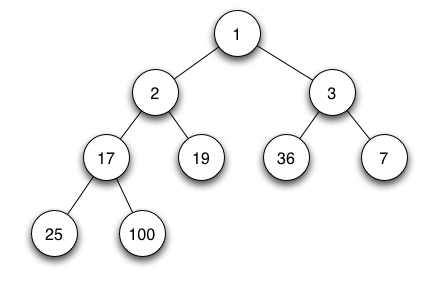
\includegraphics[width=0.6\textwidth,natwidth=442]{min-heap.png}}
  \caption{Пример заполненной кучи для минимума}
  \label{pic:min-heap}
\end{figure} 
\input{latex/HeapModule.tex}

\section{Выводы по главе \ref{chapter2}}

Разработаны типы данных для представления структуры данных двоичная куча.
